\documentclass[12pt, oneside]{book}
\usepackage[a4paper,top=2.5cm,bottom=2.5cm,left=3.5cm,right=2cm]{geometry}
\usepackage[utf8]{inputenc}
\usepackage[T1]{fontenc}
\usepackage{graphicx}
\usepackage{url}
\usepackage[hidelinks,breaklinks]{hyperref}
\usepackage[slovak]{babel} % vypnite pre prace v anglictine
\linespread{1.25} % hodnota 1.25 by mala zodpovedat 1.5 riadkovaniu

% -------------------
% --- Definicia zakladnych pojmov
% --- Vyplnte podla vasho zadania
% -------------------
\def\mfrok{2017}
\def\mfnazov{Computational Design of Probes \\for the Hyb-Seq Protocol}
\def\mftyp{Bachelor thesis}
\def\mfautor{Michaela Šandalová}
\def\mfskolitel{Mgr. Matúš Kempa}

%ak mate konzultanta, odkomentujte aj jeho meno na titulnom liste
\def\mfkonzultant{TODO}  

\def\mfmiesto{Bratislava, \mfrok}

%aj cislo odboru je povinne a je podla studijneho odboru autora prace
\def\mfodbor{2508 and 1536 Computer science and biology} 
\def\program{ Bioinformatics }
\def\mfpracovisko{ Department of Computer Science }

\begin{document}     
\frontmatter


% -------------------
% --- Obalka ------
% -------------------
\thispagestyle{empty}

\begin{center}
\sc\large
Comenius University, Bratislava\\
Faculty of Mathematics, Physics and Informatics

\vfill

{\LARGE\mfnazov}\\
\mftyp
\end{center}

\vfill

{\sc\large 
\noindent \mfrok\\
\mfautor
}

\eject % EOP i
% --- koniec obalky ----

% -------------------
% --- Titulný list
% -------------------

\thispagestyle{empty}
\noindent

\begin{center}
\sc  
\large
Comenius University, Bratislava\\
Faculty of Mathematics, Physics and Informatics

\vfill

{\LARGE\mfnazov}\\
\mftyp
\end{center}

\vfill

\noindent
\begin{tabular}{ll}
Study programme: & \program \\
Study field: & \mfodbor \\
Department: & \mfpracovisko \\
Supervisor: & \mfskolitel \\
% Konzultant: & \mfkonzultant \\
\end{tabular}

\vfill


\noindent \mfmiesto\\
\mfautor

\eject % EOP i


% --- Koniec titulnej strany


% -------------------
% --- Zadanie z AIS
% -------------------
% v tlačenej verzii s podpismi zainteresovaných osôb.
% v elektronickej verzii sa zverejňuje zadanie bez podpisov

\newpage 
\thispagestyle{empty}
\hspace{-2cm}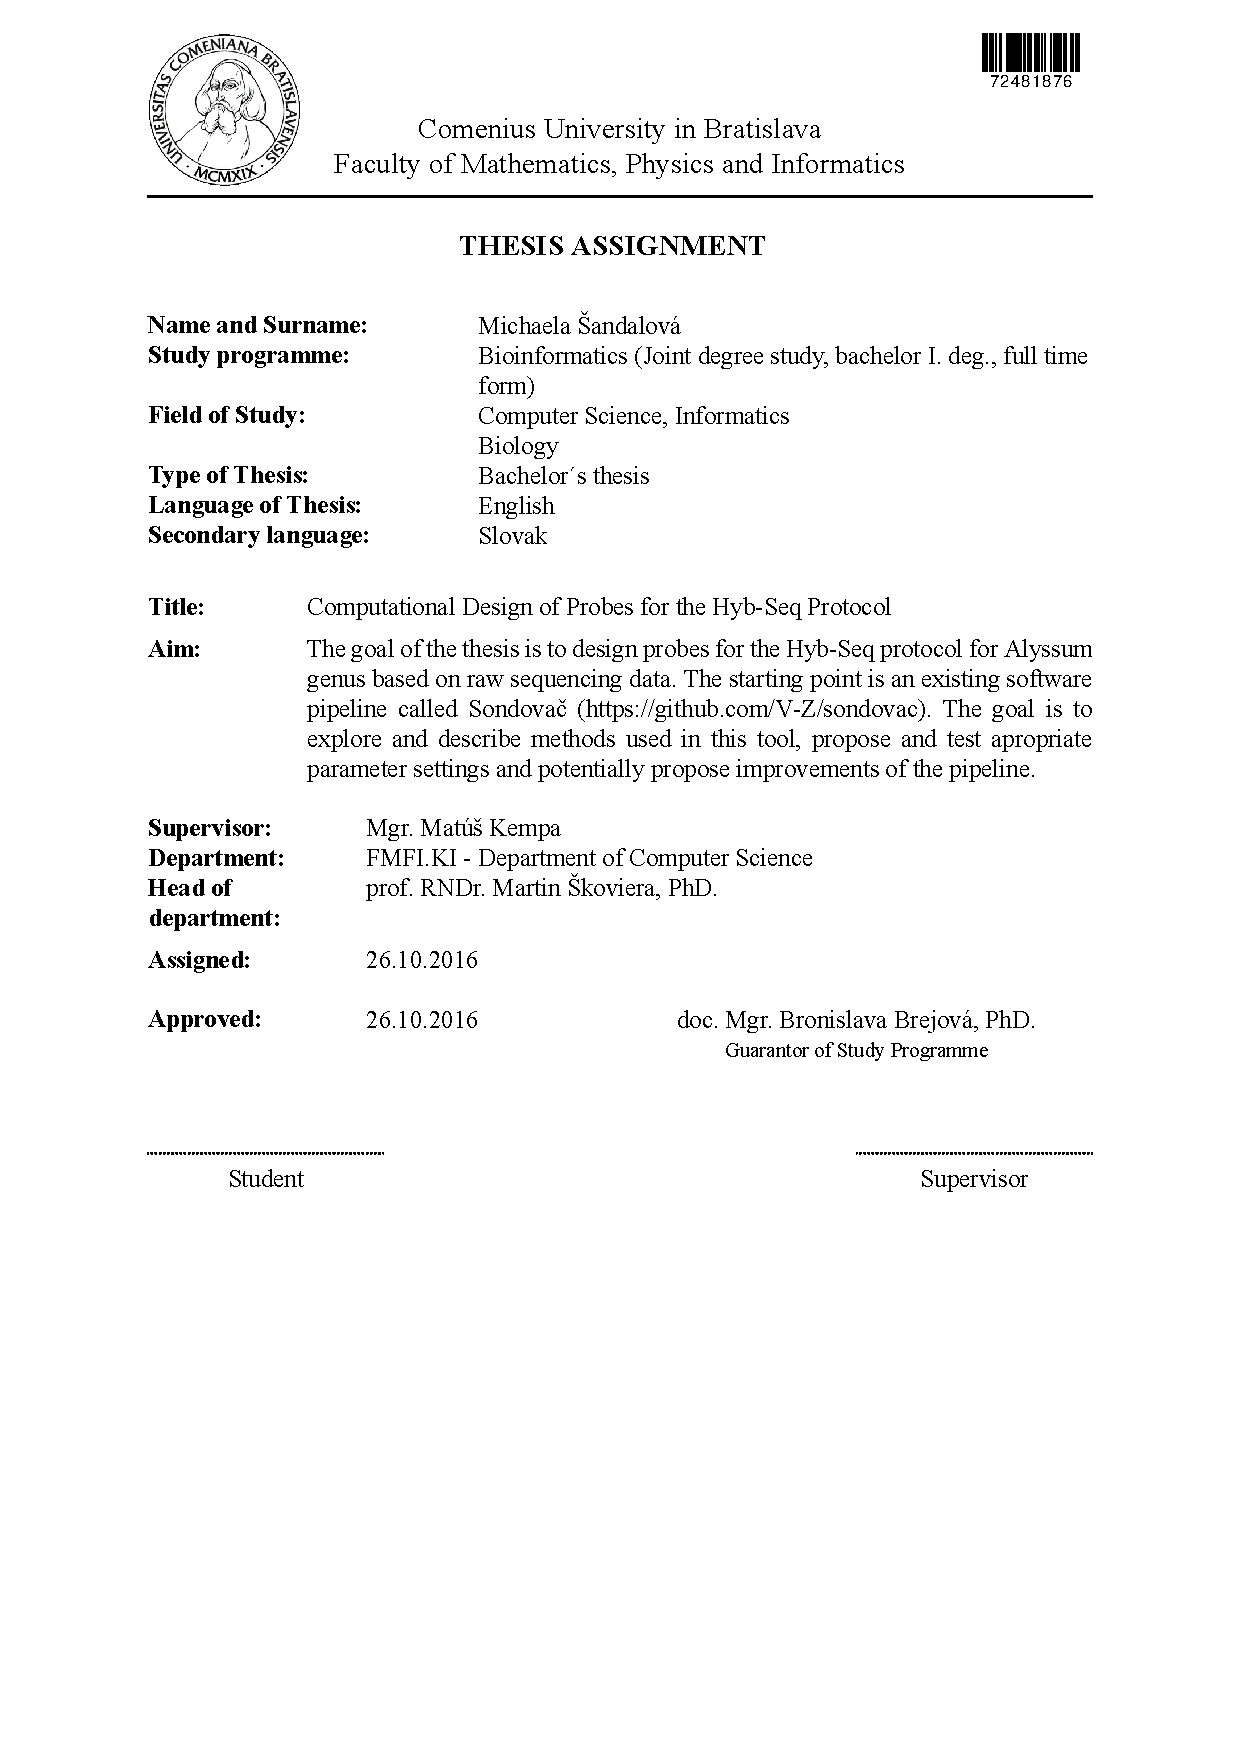
\includegraphics[width=1.1\textwidth]{images/assignment_sandalova.pdf}

\newpage 
\thispagestyle{empty}
\hspace{-2cm}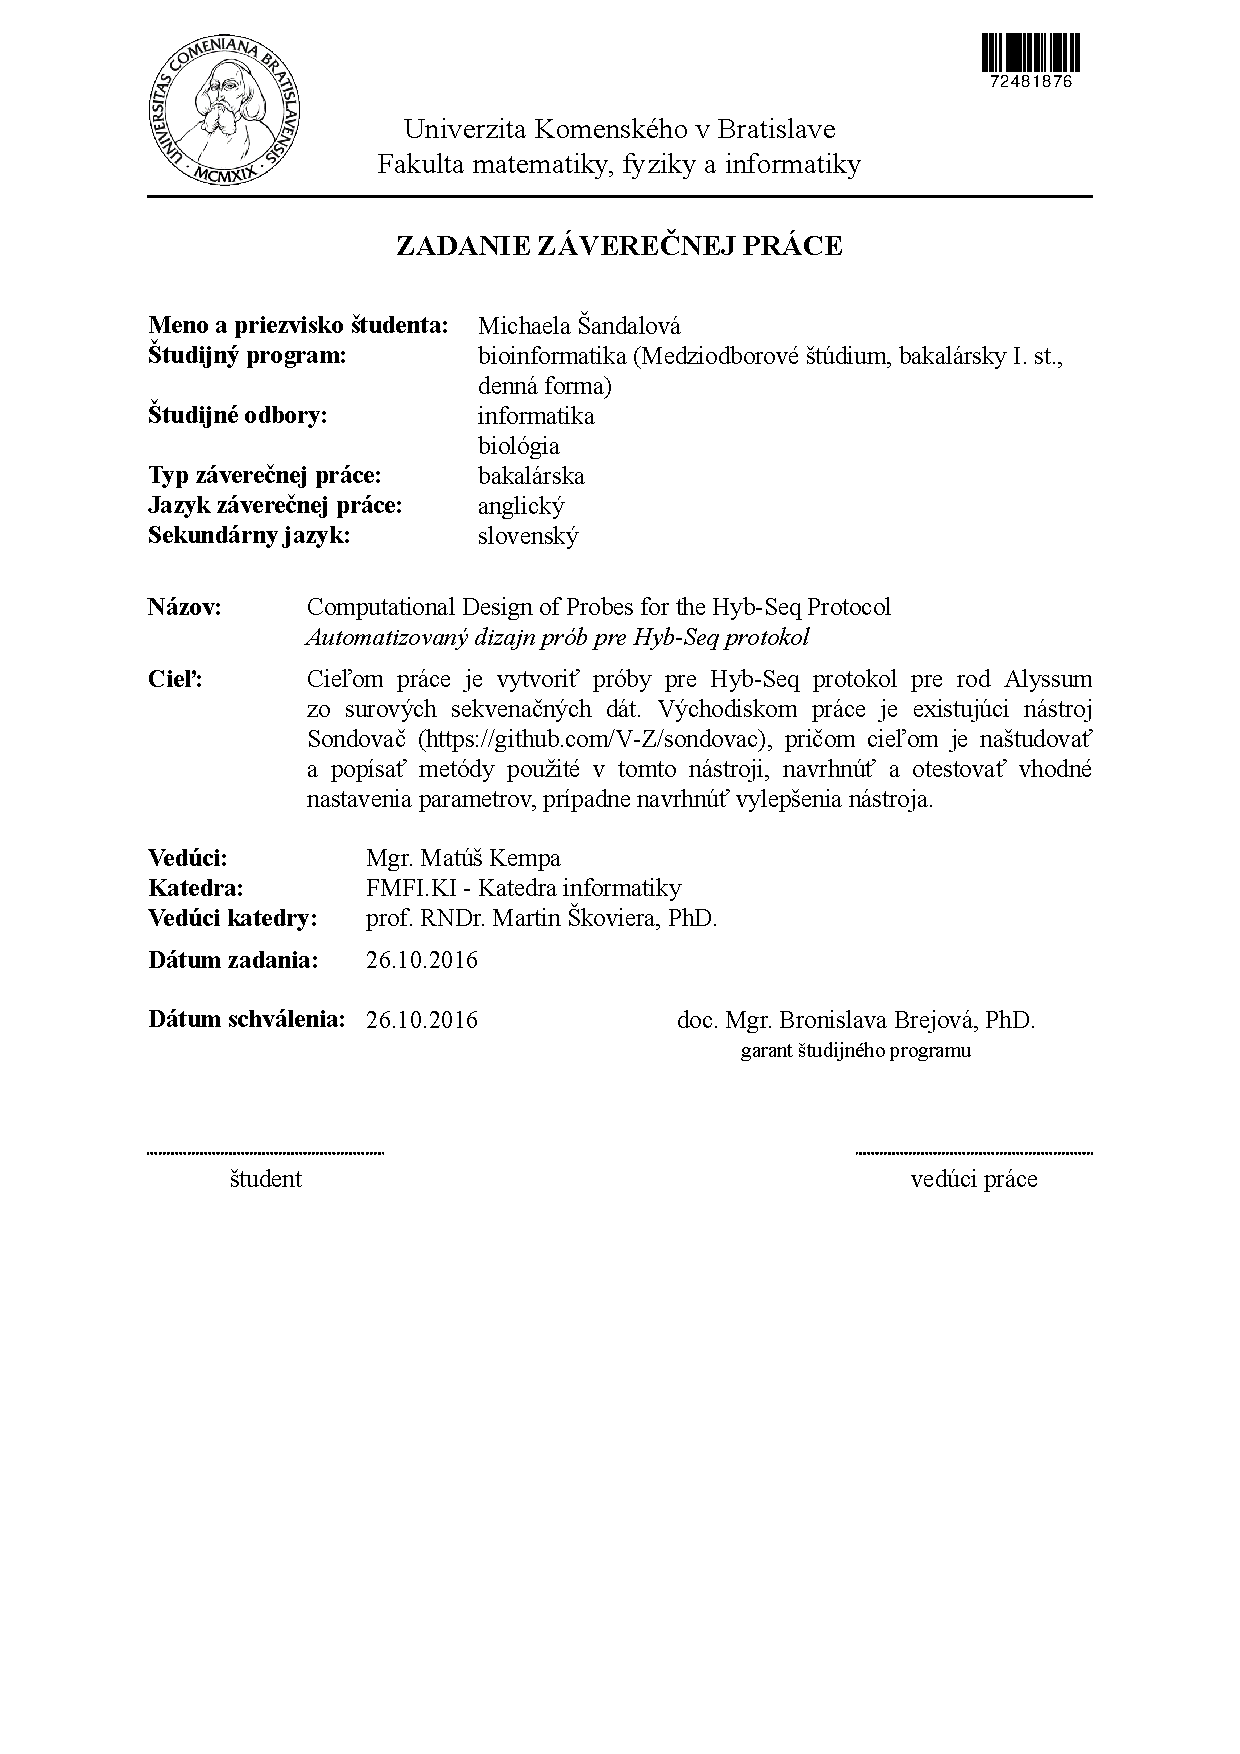
\includegraphics[width=1.1\textwidth]{images/zadanie_sandalova.pdf}

% --- Koniec zadania

\frontmatter

% -------------------
%   Poďakovanie - nepovinné
% -------------------
\setcounter{page}{3}
\newpage 
~

\vfill
{\bf Poďakovanie:} I would like to thank several people that helped me finish this thesis. 
First of all, I would like to thank my supervisor, Matúš Kempa, and his colleagues at SAV that 
answered many of my questions and allowed me to contribute to this project. 
I would also like to thank Broňa Brejová and Tomáš Vinař for helping me with making this thesis possible. 
Lastly, I would like to thank my partner and my family, who endured it all till the end. And also my dog and 
pet rats, who helped keep the morale high. 

% --- Koniec poďakovania

% -------------------
%   Abstrakt - Slovensky
% -------------------
\newpage 
\section*{Abstrakt}

Hyb-Seq protokol je prístup, ktorý umožňuje nachádzanie efektívnych genetických značiek na štúdium 
fylogenézy. Použili sme existujúci skript, Sondovač, čo je automatizované zreťazené spracovanie dát, ktoré 
vyrobí jadrové sondy s nízkym počtom kópií pre použitie v rastlinnej fylogenéze. Sondovač používa transkriptóm a genómové "skim" 
dáta a vyrobí sondy pre neskoršie použitie pri cielenom obohatení sekvencií. Vyrobili sme určité množstvo prób z dvoch počiatočných 
sád dát. Z týchto prób sme ďalej vybrali tie, ktoré sme považovali za relevantné genetické značky pomocou programu, ktorý sme napísali. 
Tento program nám pomohol naplniť požiadavky, ktoré sme na sondy mali a vybral sondy, ktoré obsahujú $1,000,000$ bázových párov. 
\paragraph*{Kľúčové slová:} Hyb-seq, sondy, fylogenéza, genetické značky 
% --- Koniec Abstrakt - Slovensky


% -------------------
% --- Abstrakt - Anglicky 
% -------------------
\newpage 
\section*{Abstract}

The Hyb-Seq protocol is na approach, that enables finding effective genetic markers for study of phylogeny. 
We used an existing script -- Sondovač -- which is an automated pipeline that creates orthologous low-copy 
nuclear probes for use in plant phylogeny. Sondovač uses transcriptome and genome skim data and creates probes 
for later target enrichment. 
We created a number of initial probes from two initial sets of plant data. From these probes we picked those we 
considered to be relevant genetic markers using a script we coded. The script helped to fulfill the 
requirements we placed on the probes and created probes that are made of $1,000,000$ base pairs. 


\paragraph*{Keywords:} Hyb-seq, probes, phylogeny, genetic markers

% --- Koniec Abstrakt - Anglicky

% -------------------
% --- Predhovor - v informatike sa zvacsa nepouziva
% -------------------
%\newpage 
%\thispagestyle{empty}
%
%\huge{Predhovor}
%\normalsize
%\newline
%Predhovor je všeobecná informácia o práci, obsahuje hlavnú charakteristiku práce 
%a okolnosti jej vzniku. Autor zdôvodní výber témy, stručne informuje o cieľoch 
%a význame práce, spomenie domáci a zahraničný kontext, komu je práca určená, 
%použité metódy, stav poznania; autor stručne charakterizuje svoj prístup a svoje 
%hľadisko. 
%
% --- Koniec Predhovor


% -------------------
% --- Obsah
% -------------------

\newpage 

\tableofcontents

% ---  Koniec Obsahu

% -------------------
% --- Zoznamy tabuliek, obrázkov - nepovinne
% -------------------

\newpage 

\listoffigures
\listoftables

% ---  Koniec Zoznamov

\mainmatter


\input introduction.tex 

\input biological_motivation.tex

%\input data_and_objectives.tex

\input hyb_seq.tex

\input existing_work.tex

\input practical_work.tex

\input results.tex

%\input improvements.tex

%\input kapitola.tex

%\input latex.tex

%\input lorem.tex

\input zaver.tex

% -------------------
% --- Bibliografia
% -------------------


\newpage	

\backmatter

\thispagestyle{empty}
\nocite{*}
\clearpage

\bibliographystyle{plain}
\bibliography{literatura} 

%Prípadne môžete napísať literatúru priamo tu
%\begin{thebibliography}{5}
 
%\bibitem{br1} MOLINA H. G. - ULLMAN J. D. - WIDOM J., 2002, Database Systems, Upper Saddle River : Prentice-Hall, 2002, 1119 s., Pearson International edition, 0-13-098043-9

%\bibitem{br2} MOLINA H. G. - ULLMAN J. D. - WIDOM J., 2000 , Databasse System implementation, New Jersey : Prentice-Hall, 2000, 653s., ???

%\bibitem{br3} ULLMAN J. D. - WIDOM J., 1997, A First Course in Database Systems, New Jersey : Prentice-Hall, 1997, 470s., 

%\bibitem{br4} PREFUSE, 2007, The Prefuse visualization toolkit,  [online] Dostupné na internete: <http://prefuse.org/>

%\bibitem{br5} PREFUSE Forum, Sourceforge - Prefuse Forum,  [online] Dostupné na internete: <http://sourceforge.net/projects/prefuse/>

%\end{thebibliography}

%---koniec Referencii

% -------------------
%--- Prilohy---
% -------------------

%Nepovinná časť prílohy obsahuje materiály, ktoré neboli zaradené priamo  do textu. Každá príloha sa začína na novej strane.
%Zoznam príloh je súčasťou obsahu.
%
%\addcontentsline{toc}{chapter}{Appendix A}
%\input AppendixA.tex
%
%\addcontentsline{toc}{chapter}{Appendix B}
%\input AppendixB.tex

\end{document}






